\begin{figure}[hb]
\begin{minipage}[h]{0.33\linewidth}
	\centering
    \vbox{ 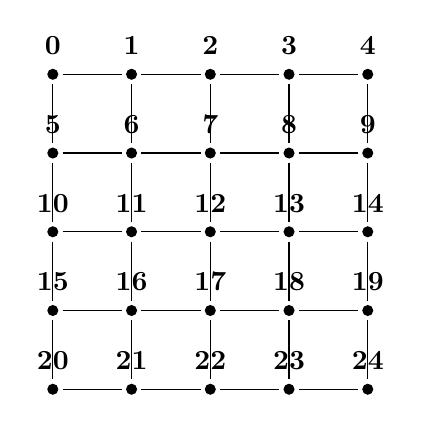
\begin{tikzpicture}
		\node[label=above:$\bf{0}$] (v0) at (0,0) {};\fill (v0) circle (2pt);
		\node[label=above:$\bf{1}$] (v1) at (1,0) {};\fill (v1) circle (2pt);
		\node[label=above:$\bf{2}$] (v2) at (2,0) {};\fill (v2) circle (2pt);
		\node[label=above:$\bf{3}$] (v3) at (3,0) {};\fill (v3) circle (2pt);
		\node[label=above:$\bf{4}$] (v4) at (4,0) {};\fill (v4) circle (2pt);
		
		\node[label=above:$\bf{5}$] (v5) at (0,-1) {};\fill (v5) circle (2pt);
		\node[label=above:$\bf{6}$] (v6) at (1,-1) {};\fill (v6) circle (2pt);
		\node[label=above:$\bf{7}$] (v7) at (2,-1) {};\fill (v7) circle (2pt);
		\node[label=above:$\bf{8}$] (v8) at (3,-1) {};\fill (v8) circle (2pt);
		\node[label=above:$\bf{9}$] (v9) at (4,-1) {};\fill (v9) circle (2pt);
	
		\node[label=above:$\bf{10}$] (v10) at (0,-2) {};\fill (v10) circle (2pt);
		\node[label=above:$\bf{11}$] (v11) at (1,-2) {};\fill (v11) circle (2pt);
		\node[label=above:$\bf{12}$] (v12) at (2,-2) {};\fill (v12) circle (2pt);
		\node[label=above:$\bf{13}$] (v13) at (3,-2) {};\fill (v13) circle (2pt);
		\node[label=above:$\bf{14}$] (v14) at (4,-2) {};\fill (v14) circle (2pt);
	
		\node[label=above:$\bf{15}$] (v15) at (0,-3) {};\fill (v15) circle (2pt);
		\node[label=above:$\bf{16}$] (v16) at (1,-3) {};\fill (v16) circle (2pt);
		\node[label=above:$\bf{17}$] (v17) at (2,-3) {};\fill (v17) circle (2pt);
		\node[label=above:$\bf{18}$] (v18) at (3,-3) {};\fill (v18) circle (2pt);
		\node[label=above:$\bf{19}$] (v19) at (4,-3) {};\fill (v19) circle (2pt);
	
		\node[label=above:$\bf{20}$] (v20) at (0,-4) {};\fill (v20) circle (2pt);
		\node[label=above:$\bf{21}$] (v21) at (1,-4) {};\fill (v21) circle (2pt);
		\node[label=above:$\bf{22}$] (v22) at (2,-4) {};\fill (v22) circle (2pt);
		\node[label=above:$\bf{23}$] (v23) at (3,-4) {};\fill (v23) circle (2pt);
		\node[label=above:$\bf{24}$] (v24) at (4,-4) {};\fill (v24) circle (2pt);
		
		\draw[-] (v0) to (v1); \draw[-]  (v0) to (v5);
		\draw[-] (v1) to (v2); \draw[-]  (v1) to (v6);
		\draw[-] (v2) to (v3); \draw[-]  (v2) to (v7);
		\draw[-] (v3) to (v4); \draw[-]  (v3) to (v8);
		\draw[-] (v4) to (v9);
		\draw[-] (v5) to (v6); \draw[-]  (v5) to (v10);
		\draw[-] (v6) to (v7); \draw[-]  (v6) to (v11);
		\draw[-] (v7) to (v8); \draw[-]  (v7) to (v12);
		\draw[-] (v8) to (v9); \draw[-]  (v8) to (v13);
		\draw[-] (v9) to (v14);
		\draw[-] (v10) to (v11); \draw[-]  (v10) to (v15);
		\draw[-] (v11) to (v12); \draw[-]  (v11) to (v16);
		\draw[-] (v12) to (v13); \draw[-]  (v12) to (v17);
		\draw[-] (v13) to (v14); \draw[-]  (v13) to (v18);
		\draw[-] (v14) to (v19);
	
		\draw[-] (v15) to (v16); \draw[-]  (v15) to (v20);
		\draw[-] (v16) to (v17); \draw[-]  (v16) to (v21);
		\draw[-] (v17) to (v18); \draw[-]  (v17) to (v22);
		\draw[-] (v18) to (v19); \draw[-]  (v18) to (v23);
		\draw[-] (v19) to (v24);
		\draw[-] (v20) to (v21);
		\draw[-] (v21) to (v22);
		\draw[-] (v22) to (v23);
		\draw[-] (v23) to (v24);
    \end{tikzpicture}}
\end{minipage}
\hfill
\begin{minipage}[h]{0.33\linewidth}
	\centering
    \vbox{ 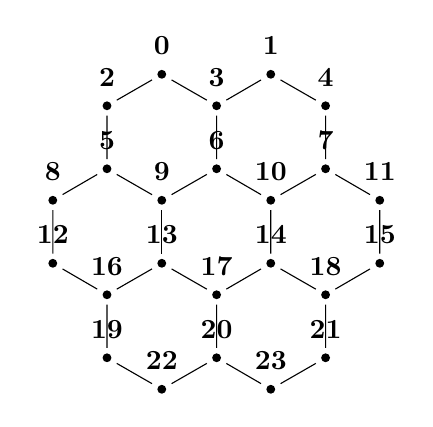
\begin{tikzpicture}[scale=0.8]
		\node[label=above:$\bf{0}$] (v0) at (0,0) {};\fill (v0) circle (2pt);
		\node[label=above:$\bf{1}$] (v1) at (1.73,0) {};\fill (v1) circle (2pt);

		\node[label=above:$\bf{2}$] (v2) at (-0.87,-0.5) {};\fill (v2) circle (2pt);
		\node[label=above:$\bf{3}$] (v3) at (0.87,-0.5) {};\fill (v3) circle (2pt);
		\node[label=above:$\bf{4}$] (v4) at (2.6,-0.5) {};\fill (v4) circle (2pt);
		
		\node[label=above:$\bf{5}$] (v5) at (-0.87,-1.5) {};\fill (v5) circle (2pt);
		\node[label=above:$\bf{6}$] (v6) at (0.87,-1.5) {};\fill (v6) circle (2pt);
		\node[label=above:$\bf{7}$] (v7) at (2.6,-1.5) {};\fill (v7) circle (2pt);

		\node[label=above:$\bf{8}$] (v8) at (-1.73,-2) {};\fill (v8) circle (2pt);
		\node[label=above:$\bf{9}$] (v9) at (0,-2) {};\fill (v9) circle (2pt);
		\node[label=above:$\bf{10}$] (v10) at (1.73,-2) {};\fill (v10) circle (2pt);
		\node[label=above:$\bf{11}$] (v11) at (3.46,-2) {};\fill (v11) circle (2pt);

		\node[label=above:$\bf{12}$] (v12) at (-1.73,-3) {};\fill (v12) circle (2pt);
		\node[label=above:$\bf{13}$] (v13) at (0,-3) {};\fill (v13) circle (2pt);
		\node[label=above:$\bf{14}$] (v14) at (1.73,-3) {};\fill (v14) circle (2pt);
		\node[label=above:$\bf{15}$] (v15) at (3.46,-3) {};\fill (v15) circle (2pt);

		\node[label=above:$\bf{16}$] (v16) at (-0.87,-3.5) {};\fill (v16) circle (2pt);
		\node[label=above:$\bf{17}$] (v17) at (0.87,-3.5) {};\fill (v17) circle (2pt);
		\node[label=above:$\bf{18}$] (v18) at (2.6,-3.5) {};\fill (v18) circle (2pt);

		\node[label=above:$\bf{19}$] (v19) at (-0.87,-4.5) {};\fill (v19) circle (2pt);
		\node[label=above:$\bf{20}$] (v20) at (0.87,-4.5) {};\fill (v20) circle (2pt);
		\node[label=above:$\bf{21}$] (v21) at (2.6,-4.5) {};\fill (v21) circle (2pt);

		\node[label=above:$\bf{22}$] (v22) at (0,-5) {};\fill (v22) circle (2pt);
		\node[label=above:$\bf{23}$] (v23) at (1.73,-5) {};\fill (v23) circle (2pt);

		
		\draw[-] (v0) to (v2); \draw[-]  (v0) to (v3);
		\draw[-] (v1) to (v3); \draw[-]  (v1) to (v4);
		\draw[-] (v2) to (v5); 
		\draw[-] (v3) to (v6);
		\draw[-] (v4) to (v7);
		\draw[-] (v5) to (v8); \draw[-] (v5) to (v9);
		\draw[-] (v6) to (v9); \draw[-] (v6) to (v10);
		\draw[-] (v7) to (v10);\draw[-] (v7) to (v11);
		\draw[-] (v8) to (v12);
		\draw[-] (v9) to (v13);
		\draw[-] (v10) to (v14);
		\draw[-] (v11) to (v15);
		\draw[-] (v12) to (v16);
		\draw[-] (v13) to (v16); \draw[-] (v13) to (v17);
		\draw[-] (v14) to (v17); \draw[-] (v14) to (v18);
		\draw[-] (v15) to (v18);
		\draw[-] (v16) to (v19);
		\draw[-] (v17) to (v20);
		\draw[-] (v18) to (v21);
		\draw[-] (v19) to (v22);
		\draw[-] (v20) to (v22); \draw[-] (v20) to (v23);
		\draw[-] (v21) to (v23);
    \end{tikzpicture}}
\end{minipage}
\hfill
\begin{minipage}[h]{0.33\linewidth}
	\centering
    \vbox{ 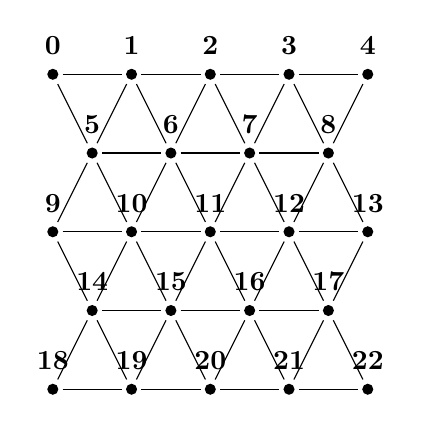
\begin{tikzpicture}
		\node[label=above:$\bf{0}$] (v0) at (0,0) {};\fill (v0) circle (2pt);
		\node[label=above:$\bf{1}$] (v1) at (1,0) {};\fill (v1) circle (2pt);
		\node[label=above:$\bf{2}$] (v2) at (2,0) {};\fill (v2) circle (2pt);
		\node[label=above:$\bf{3}$] (v3) at (3,0) {};\fill (v3) circle (2pt);
		\node[label=above:$\bf{4}$] (v4) at (4,0) {};\fill (v4) circle (2pt);
		
		\node[label=above:$\bf{5}$] (v5) at (0.5,-1) {};\fill (v5) circle (2pt);
		\node[label=above:$\bf{6}$] (v6) at (1.5,-1) {};\fill (v6) circle (2pt);
		\node[label=above:$\bf{7}$] (v7) at (2.5,-1) {};\fill (v7) circle (2pt);
		\node[label=above:$\bf{8}$] (v8) at (3.5,-1) {};\fill (v8) circle (2pt);
	
		\node[label=above:$\bf{9}$] (v9) at (0,-2) {};\fill (v9) circle (2pt);
		\node[label=above:$\bf{10}$] (v10) at (1,-2) {};\fill (v10) circle (2pt);
		\node[label=above:$\bf{11}$] (v11) at (2,-2) {};\fill (v11) circle (2pt);
		\node[label=above:$\bf{12}$] (v12) at (3,-2) {};\fill (v12) circle (2pt);
		\node[label=above:$\bf{13}$] (v13) at (4,-2) {};\fill (v13) circle (2pt);
	
		\node[label=above:$\bf{14}$] (v14) at (0.5,-3) {};\fill (v14) circle (2pt);
		\node[label=above:$\bf{15}$] (v15) at (1.5,-3) {};\fill (v15) circle (2pt);
		\node[label=above:$\bf{16}$] (v16) at (2.5,-3) {};\fill (v16) circle (2pt);
		\node[label=above:$\bf{17}$] (v17) at (3.5,-3) {};\fill (v17) circle (2pt);

	
		\node[label=above:$\bf{18}$] (v18) at (0,-4) {};\fill (v18) circle (2pt);
		\node[label=above:$\bf{19}$] (v19) at (1,-4) {};\fill (v19) circle (2pt);
		\node[label=above:$\bf{20}$] (v20) at (2,-4) {};\fill (v20) circle (2pt);
		\node[label=above:$\bf{21}$] (v21) at (3,-4) {};\fill (v21) circle (2pt);
		\node[label=above:$\bf{22}$] (v22) at (4,-4) {};\fill (v22) circle (2pt);
		
		\draw[-] (v0) to (v1); \draw[-]  (v0) to (v5);
		\draw[-] (v1) to (v2); \draw[-]  (v1) to (v5); \draw[-]  (v1) to (v6);
		\draw[-] (v2) to (v3); \draw[-]  (v2) to (v6); \draw[-]  (v2) to (v7);
		\draw[-] (v3) to (v4); \draw[-]  (v3) to (v7); \draw[-]  (v3) to (v8);
		\draw[-] (v4) to (v8);
		\draw[-] (v5) to (v6); \draw[-]  (v5) to (v9); \draw[-]  (v5) to (v10);
		\draw[-] (v6) to (v7); \draw[-]  (v6) to (v10); \draw[-]  (v6) to (v11);
		\draw[-] (v7) to (v8); \draw[-]  (v7) to (v11); \draw[-]  (v7) to (v12);
		\draw[-] (v8) to (v12); \draw[-]  (v8) to (v13);
		\draw[-] (v9) to (v10); \draw[-] (v9) to (v14);
		\draw[-] (v10) to (v11); \draw[-]  (v10) to (v14);\draw[-]  (v10) to (v15);
		\draw[-] (v11) to (v12); \draw[-]  (v11) to (v15);\draw[-]  (v11) to (v16);
		\draw[-] (v12) to (v13); \draw[-]  (v12) to (v16);\draw[-]  (v12) to (v17);
		\draw[-]  (v13) to (v17);
		\draw[-] (v14) to (v15); \draw[-] (v14) to (v18); \draw[-] (v14) to (v19);
		\draw[-] (v15) to (v16); \draw[-] (v15) to (v19); \draw[-] (v15) to (v20);
		\draw[-] (v16) to (v17); \draw[-] (v16) to (v20); \draw[-] (v16) to (v21);
		\draw[-] (v17) to (v21); \draw[-] (v17) to (v22);
		\draw[-] (v18) to (v19);
		\draw[-] (v19) to (v20);
		\draw[-] (v20) to (v21);
		\draw[-] (v21) to (v22);
    \end{tikzpicture}}
\end{minipage}
\begin{minipage}[ht]{1\linewidth}
\begin{tabular}{p{0.32\linewidth}p{0.32\linewidth}p{0.32\linewidth}}
\centering a) Square Lattice & \centering b) Hexagonal Lattice  & \centering c) Triangular Lattice \\
\end{tabular}
\end{minipage}
\caption{ Examples of lattice graphs}
\label{fig:2}
\end{figure}